\documentclass[14pt,a4paper,report]{ncc}
\usepackage[a4paper, mag=1000, left=2.5cm, right=1cm, top=2cm, bottom=2cm, headsep=0.7cm, footskip=1cm]{geometry}
\usepackage[utf8]{inputenc}
\usepackage[english,russian]{babel}
\usepackage{indentfirst}
\usepackage[dvipsnames]{xcolor}
\usepackage[colorlinks]{hyperref}
\usepackage{listings} 
\usepackage{caption}
\DeclareCaptionFont{white}{\color{white}} 
\DeclareCaptionFormat{listing}{\colorbox{gray}{\parbox{\textwidth}{#1#2#3}}}
\captionsetup[lstlisting]{format=listing,labelfont=white,textfont=white}
\lstset{% Собственно настройки вида листинга
inputencoding=utf8, extendedchars=\true, keepspaces = true, % поддержка кириллицы и пробелов в комментариях
language=C++,            % выбор языка для подсветки (здесь это Pascal)
basicstyle=\small\sffamily, % размер и начертание шрифта для подсветки кода
numbers=left,               % где поставить нумерацию строк (слева\справа)
numberstyle=\tiny,          % размер шрифта для номеров строк
stepnumber=1,               % размер шага между двумя номерами строк
numbersep=5pt,              % как далеко отстоят номера строк от подсвечиваемого кода
backgroundcolor=\color{white}, % цвет фона подсветки - используем \usepackage{color}
showspaces=false,           % показывать или нет пробелы специальными отступами
showstringspaces=false,     % показывать или нет пробелы в строках
showtabs=false,             % показывать или нет табуляцию в строках
frame=single,               % рисовать рамку вокруг кода
tabsize=2,                  % размер табуляции по умолчанию равен 2 пробелам
captionpos=t,               % позиция заголовка вверху [t] или внизу [b] 
breaklines=true,            % автоматически переносить строки (да\нет)
breakatwhitespace=false,    % переносить строки только если есть пробел
escapeinside={\%*}{*)}      % если нужно добавить комментарии в коде
}

\begin{document}
% Переоформление некоторых стандартных названий
\renewcommand{\chaptername}{Лабораторная работа}
\def\contentsname{Содержание}

% Оформление титульного листа
\begin{titlepage}
\begin{center}
\textsc{Министерство образования и науки Украины\\[2mm]
Государственный университет телекомуникаций\\[5mm]
Учебно-научный институт Телекомуникаций и информатизации\\[2mm]
Кафедра компьютерной инженерии}

\vfill

\textbf{ОТЧЁТ ПО ЛАБОРАТОРНЫМ РАБОТАМ\\[3mm]
курса «Системное Прогпрамное Обеспечение»\\[6mm]
Вариант 13
\\[20mm]
}
\end{center}

\hfill
\begin{minipage}{.5\textwidth}
Выполнил студент:\\[2mm] 
Максимов Евгений Сергеевич\\
группа: КИД-21\\[5mm]

Проверил:\\[2mm] 
старший преподователь\\
Кучеренко Владимир Николаевич
\end{minipage}%
\vfill
\begin{center}
 Киев, \theyear\ г.
\end{center}
\end{titlepage}

% Содержание
\tableofcontents
\newpage

\chapter{Сеанс работы в Linux}

\section{Задание}
	Определение понятий и анализ работы ниже названных объектов и процессов, которые происходят при сеансе работы в Linux:
\begin{itemize}
	\item Загрузка системы, ядро ​​системы, регистрация в системе, имя входящего пользователя.
	\item Персональный компьютер, многопользовательская операционная система, 					пользователи, администраторы, домашний каталог.
	\item Учетная запись UID, GID, полное имя, командная оболочка, интерпретатор командной 	строки, задачи администратора и его UID и GID.
	\item Хост, пароль, приглашение командной строки, идентификация.
	\item Виртуальные консоли их интерфейс, вызов виртуальных консолей и работа в них.
	\item Графические консоли.
	\item Имя пользователя, сеанс работы в системе, выходной поток данных, выход из 			системы.
\end{itemize}
\section{Основная часть}
	Обработка работы команд:
\begin{enumerate}
	\item Регистрация в системе.
	\begin{figure}[h]
		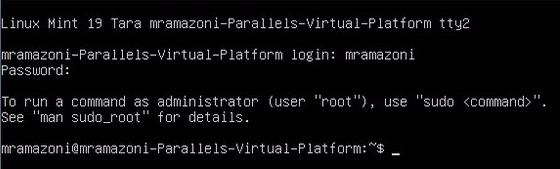
\includegraphics{lab1_2.png}
		\centering
	\end{figure}
	\newpage
	\item Изменение пароля.
	\begin{figure}[h]
		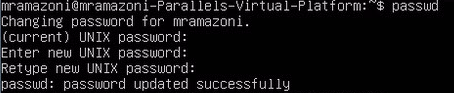
\includegraphics{lab1_3.png}
		\centering
	\end{figure}
	\item Определение учетной записи пользователя от имени которого выполняется работа.
	\begin{figure}[h]
		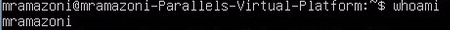
\includegraphics{lab1_4.png}
		\centering
	\end{figure}
	\item Вывод списка пользователей, которые в данный момент зарегистрированы в системе.
	\begin{figure}[h]
		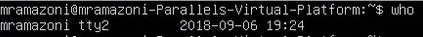
\includegraphics{lab1_5.png}
		\centering
	\end{figure}
	\item Вывод информации о пользователях, работавших в системе.
	\begin{figure}[h]
		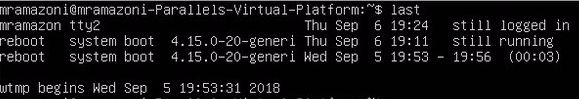
\includegraphics{lab1_6.png}
		\centering
	\end{figure}
	\item Выход из системы.
	\begin{figure}[h]
		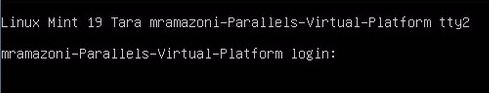
\includegraphics{lab1_1.png}
		\centering
	\end{figure}
\end{enumerate}

\section{Выводы}


%\input{lab2} Отчёт к каждой работе оформляется в отдельном файле


\end{document}